\section{Proposed Method}
\label{sec:method}
\begin{figure*}[t]
 \centering
 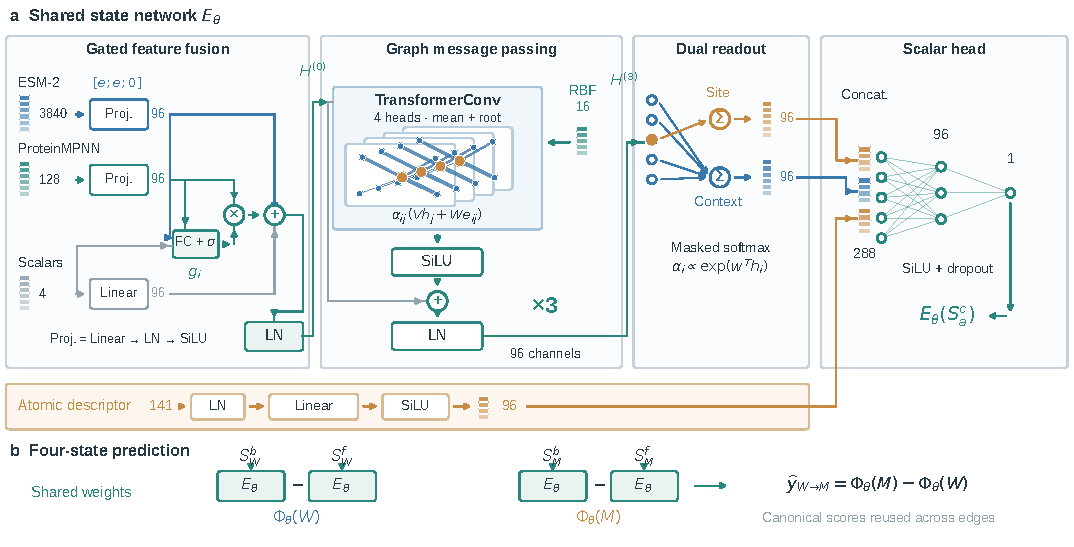
\includegraphics[width=\textwidth]{fig_model.pdf}
 \caption{DiMA-PPI network architecture. (a) Projected sequence and backbone
 features enter a learned sigmoid gate; elementwise multiplication and addition
 form the fused node features. Each of three graph blocks contains four-head
 TransformerConv, SiLU, a residual addition and LayerNorm (LN). Edge RBFs enter
 attention; line widths schematically indicate attention weights. Masked
 attention pools the mutation site and context separately. Their two 96-D
 vectors are concatenated with a projected 96-D atomic descriptor and passed
 through a 288--96--1 scalar head. Drawn neurons represent layers rather than
 exact neuron counts. (b) The same network scores all four bound/free and
 WT/mutant states. Bound-minus-free scores define binding potentials, whose
 difference gives the mutation effect. Canonical scores are reused across edges.}
 \label{fig:model}
\end{figure*}
Figure~\ref{fig:model} summarizes the shared encoder, four-state output and
canonical inference procedure.
\subsection{Canonical Bound and Free States}
For a fixed complex and substitution site, $S_a$ denotes the state with
amino-acid identity $a$. Positive $y_{a\to b}=\Delta\Delta G_{a\to b}$ follows
the benchmark convention of stronger mutant binding. Each state has a bound
context $S_a^b$ and an isolated-chain free context $S_a^f$, identified by
\begin{equation}
 k(a,c)=(\text{complex},\text{chain},\text{PDB site},a,c),
 \quad c\in\{b,f\}.
\end{equation}
Each key maps to one representation selected by source-row order,
independently of labels and fold assignments. Repeated occurrences reuse
identical sequence features, graph geometry, node masks and atomic
descriptors, ensuring a consistent representation of shared intermediate
states.

The reference-backbone graph contains residues within 20~\AA{} of the site.
Edges connect residues within 8~\AA{} and sequential neighbors on each chain;
16 radial basis functions encode their distances. The bound encoder uses the
complex graph. For the free context, cross-chain edges are removed and readout
is restricted to the mutated chain. Four 141-dimensional descriptors encode
wild-type/mutant and bound/free atomic environments. PyRosetta~\cite{pyrosetta} locally repacks
side chains within 8~\AA{} in the bound structures and repacks the isolated
mutated chain for the free contexts. Descriptors contain element-distance
histograms, substituted-residue element counts, 18 residue-level Rosetta score
terms and their local sums.

\subsection{Shared Multimodal Graph Encoder}
Each residue has an ESM-2 650M embedding $e_i^a\in\mathbb{R}^{1280}$~\cite{esm2},
a ProteinMPNN reference-backbone feature $p_i\in\mathbb{R}^{128}$~\cite{proteinmpnn},
and four scalars $s_i$ encoding chain membership, site membership and
normalized site distance. The single-state sequence block is
$u_i^a=[e_i^a;e_i^a;\mathbf{0}]$, which represents a single sequence identity
in both embedding blocks and fixes the difference block to zero.
A learned gate integrates the sequence and structural features:
\begin{align}
 q_i&=\phi_{\rm seq}(u_i^a),\quad t_i=\phi_{\rm str}(p_i),\nonumber\\
 g_i&=\sigma(W_g[q_i;t_i;s_i]+b_g),\nonumber\\
 h_i^{(0)}&=\operatorname{LN}(q_i+g_i\odot t_i+W_s s_i+b_s).
\end{align}
The projections use linear layers, layer normalization and SiLU. Three
TransformerConv layers with four averaged attention heads and hidden width
96 propagate messages over the context-specific edges:
\begin{equation}
 H^{(\ell+1)}=\operatorname{LN}\!\left[H^{(\ell)}+
 \operatorname{SiLU}\big(\operatorname{TConv}_{\ell}
 (H^{(\ell)},\mathcal E_c,R)\big)\right].
\end{equation}
Attention pooling produces separate representations of the substitution
site and surrounding context, with weights proportional to
$\exp(w^\top h_i^{(3)})$ within each node set. A shared scalar head maps these
representations and the atomic descriptor to a state score:
\begin{equation}
 E_\theta(S_a^c)=\operatorname{MLP}_\theta
 ([z_{\rm site};z_{\rm context};\phi_d(d_a^c)]),
\end{equation}
where $\phi_d$ normalizes and projects the atomic descriptor to width 96.
All four evaluations share encoder, projection and scalar-head weights.

\subsection{Potential Differences and Numerical Identity}
Define the latent binding potential and mutation prediction as
\begin{align}
 \Phi_\theta(a)&=E_\theta(S_a^b)-E_\theta(S_a^f),\\
 \widehat y_{a\to b}&=\Phi_\theta(b)-\Phi_\theta(a).
 \label{eq:potential}
\end{align}
For any path, intermediate potentials cancel:
\begin{equation}
 \sum_{\ell=0}^{L-1}\widehat y_{a_\ell\to a_{\ell+1}}
 =\Phi_\theta(a_L)-\Phi_\theta(a_0).
 \label{eq:telescoping}
\end{equation}
Equation~\eqref{eq:telescoping} establishes antisymmetry, path independence
and zero cycle sums. For an oriented node--edge incidence matrix $B$, the
prediction vector is $B^\top\boldsymbol\Phi$, a discrete potential-difference
field with zero circulation. In comparison, pairwise antisymmetrization
$[f(a,b)-f(b,a)]/2$ constrains the reversal relation.

Canonical inference preserves the state identity required by
Eq.~\eqref{eq:telescoping}. With dropout disabled, each context score can be
computed once per checkpoint and reused across all incident edges.
For stochastic inference, the same state estimate is reused within each
draw. Both procedures preserve cancellation to floating-point precision.
Mutation-effect supervision determines potential differences; a common
additive offset leaves every prediction invariant. The represented state
space is defined by the complex, substitution site and structural context.

\subsection{Optimization}
The model is optimized using observed forward mutation effects. With the
training-subset target standard deviation
$\sigma_y$ and scaled four-state output $\widetilde y_\theta$, the objective is
\begin{equation}
 \mathcal L=\frac{1}{N}\sum_n\operatorname{SmoothL1}_{0.5}
 (\widetilde y_\theta(a_n,b_n)-y_n/\sigma_y).
\end{equation}
Predictions are rescaled to physical units by multiplication with
$\sigma_y$, with the additive offset fixed at zero. The objective consists
solely of the forward-prediction loss; consistency is imposed by the output
parameterization. AdamW uses learning rate $5\times10^{-4}$,
weight decay $10^{-4}$, batch size 8 and dropout 0.15. Training runs for up to
60 epochs with validation-MSE early stopping and patience 10.
